\message{ !name(ccarroll_et_al_scipy_2018.tex)}\documentclass[10pt,twocolumn]{article}
\providecommand{\EconARK}{\href{http://econ-ark.org}{Econ-ARK}}
\usepackage{moreverb}
\usepackage{lmodern}
\usepackage{amssymb,amsmath}
\usepackage{ifxetex,ifluatex}
\usepackage{fixltx2e} % provides \textsubscript
\ifnum 0\ifxetex 1\fi\ifluatex 1\fi=0 % if pdftex
  \usepackage[T1]{fontenc}
  \usepackage[utf8]{inputenc}
\else % if luatex or xelatex
  \ifxetex
    \usepackage{mathspec}
  \else
    \usepackage{fontspec}
  \fi
  \defaultfontfeatures{Ligatures=TeX,Scale=MatchLowercase}
\fi
% use upquote if available, for straight quotes in verbatim environments
\IfFileExists{upquote.sty}{\usepackage{upquote}}{}
% use microtype if available
\IfFileExists{microtype.sty}{%
\usepackage{microtype}
\UseMicrotypeSet[protrusion]{basicmath} % disable protrusion for tt fonts
}{}
%\usepackage[margin=0.68in]{geometry}
\usepackage{hyperref}
\hypersetup{unicode=true,
            pdftitle={The Heterogeneous-Agent Resources toolKit (HARK): An Extensible Framework for Solving and Estimating Heterogeneous-Agent Economic Models},
            pdfauthor={Christopher D. Carroll; Alexander M. Kaufman; Jacqueline Kazil; David C. Low; Nathan M. Palmer; Matthew N. White},
            pdfborder={0 0 0},
            breaklinks=true}
\urlstyle{same}  % don't use monospace font for urls
\usepackage{color}
\usepackage{fancyvrb}
\newcommand{\VerbBar}{|}
\newcommand{\VERB}{\Verb[commandchars=\\\{\}]}
\DefineVerbatimEnvironment{Highlighting}{Verbatim}{commandchars=\\\{\}}
% Add ',fontsize=\small' for more characters per line
\usepackage{framed}
\definecolor{shadecolor}{RGB}{248,248,248}
\newenvironment{Shaded}{\begin{snugshade}}{\end{snugshade}}
\newcommand{\KeywordTok}[1]{\textcolor[rgb]{0.13,0.29,0.53}{\textbf{#1}}}
\newcommand{\DataTypeTok}[1]{\textcolor[rgb]{0.13,0.29,0.53}{#1}}
\newcommand{\DecValTok}[1]{\textcolor[rgb]{0.00,0.00,0.81}{#1}}
\newcommand{\BaseNTok}[1]{\textcolor[rgb]{0.00,0.00,0.81}{#1}}
\newcommand{\FloatTok}[1]{\textcolor[rgb]{0.00,0.00,0.81}{#1}}
\newcommand{\ConstantTok}[1]{\textcolor[rgb]{0.00,0.00,0.00}{#1}}
\newcommand{\CharTok}[1]{\textcolor[rgb]{0.31,0.60,0.02}{#1}}
\newcommand{\SpecialCharTok}[1]{\textcolor[rgb]{0.00,0.00,0.00}{#1}}
\newcommand{\StringTok}[1]{\textcolor[rgb]{0.31,0.60,0.02}{#1}}
\newcommand{\VerbatimStringTok}[1]{\textcolor[rgb]{0.31,0.60,0.02}{#1}}
\newcommand{\SpecialStringTok}[1]{\textcolor[rgb]{0.31,0.60,0.02}{#1}}
\newcommand{\ImportTok}[1]{#1}
\newcommand{\CommentTok}[1]{\textcolor[rgb]{0.56,0.35,0.01}{\textit{#1}}}
\newcommand{\DocumentationTok}[1]{\textcolor[rgb]{0.56,0.35,0.01}{\textbf{\textit{#1}}}}
\newcommand{\AnnotationTok}[1]{\textcolor[rgb]{0.56,0.35,0.01}{\textbf{\textit{#1}}}}
\newcommand{\CommentVarTok}[1]{\textcolor[rgb]{0.56,0.35,0.01}{\textbf{\textit{#1}}}}
\newcommand{\OtherTok}[1]{\textcolor[rgb]{0.56,0.35,0.01}{#1}}
\newcommand{\FunctionTok}[1]{\textcolor[rgb]{0.00,0.00,0.00}{#1}}
\newcommand{\VariableTok}[1]{\textcolor[rgb]{0.00,0.00,0.00}{#1}}
\newcommand{\ControlFlowTok}[1]{\textcolor[rgb]{0.13,0.29,0.53}{\textbf{#1}}}
\newcommand{\OperatorTok}[1]{\textcolor[rgb]{0.81,0.36,0.00}{\textbf{#1}}}
\newcommand{\BuiltInTok}[1]{#1}
\newcommand{\ExtensionTok}[1]{#1}
\newcommand{\PreprocessorTok}[1]{\textcolor[rgb]{0.56,0.35,0.01}{\textit{#1}}}
\newcommand{\AttributeTok}[1]{\textcolor[rgb]{0.77,0.63,0.00}{#1}}
\newcommand{\RegionMarkerTok}[1]{#1}
\newcommand{\InformationTok}[1]{\textcolor[rgb]{0.56,0.35,0.01}{\textbf{\textit{#1}}}}
\newcommand{\WarningTok}[1]{\textcolor[rgb]{0.56,0.35,0.01}{\textbf{\textit{#1}}}}
\newcommand{\AlertTok}[1]{\textcolor[rgb]{0.94,0.16,0.16}{#1}}
\newcommand{\ErrorTok}[1]{\textcolor[rgb]{0.64,0.00,0.00}{\textbf{#1}}}
\newcommand{\NormalTok}[1]{#1}
\usepackage{graphicx,grffile}
\makeatletter
\def\maxwidth{\ifdim\Gin@nat@width>\linewidth\linewidth\else\Gin@nat@width\fi}
\def\maxheight{\ifdim\Gin@nat@height>\textheight\textheight\else\Gin@nat@height\fi}
\makeatother
% Scale images if necessary, so that they will not overflow the page
% margins by default, and it is still possible to overwrite the defaults
% using explicit options in \includegraphics[width, height, ...]{}
\setkeys{Gin}{width=\maxwidth,height=\maxheight,keepaspectratio}
\IfFileExists{parskip.sty}{%
\usepackage{parskip}
}{% else
\setlength{\parindent}{0pt}
\setlength{\parskip}{6pt plus 2pt minus 1pt}
}
\setlength{\emergencystretch}{3em}  % prevent overfull lines
\providecommand{\tightlist}{%
  \setlength{\itemsep}{0pt}\setlength{\parskip}{0pt}}
\setcounter{secnumdepth}{5}
% Redefines (sub)paragraphs to behave more like sections
\ifx\paragraph\undefined\else
\let\oldparagraph\paragraph
\renewcommand{\paragraph}[1]{\oldparagraph{#1}\mbox{}}
\fi
\ifx\subparagraph\undefined\else
\let\oldsubparagraph\subparagraph
\renewcommand{\subparagraph}[1]{\oldsubparagraph{#1}\mbox{}}
\fi

%%% Use protect on footnotes to avoid problems with footnotes in titles
\let\rmarkdownfootnote\footnote%
\def\footnote{\protect\rmarkdownfootnote}

%%% Change title format to be more compact
\usepackage{titling}

% Create subtitle command for use in maketitle
\newcommand{\subtitle}[1]{
  \posttitle{
    \begin{center}\large#1\end{center}
    }
}

\setlength{\droptitle}{-2em}
  \title{The \EconARK~Open Source Tools \\ for Computational Economics}
  \pretitle{\vspace{\droptitle}\centering\huge}
  \posttitle{\par}
  \author{Christopher D. Carroll \\ Alexander M. Kaufman \\ Jacqueline Kazil \\ David C. Low \\ Nathan M. Palmer \\ Matthew N. White}
  \preauthor{\centering\large\emph}
  \postauthor{\par}
  \predate{\centering\large\emph}
  \postdate{\par}
  \date{July 9, 2018}

\usepackage{cancel}
\usepackage{fancyhdr}
\pagestyle{fancy}
\usepackage[round]{natbib}

\begin{document}

\message{ !name(ccarroll_et_al_scipy_2018.tex) !offset(-3) }

\maketitle
\begin{abstract}
  The Economics Algorithmic Repository and toolKit (Econ-ARK) aims to become a focal resource for computational economics. Its first `framework,' the Heterogeneous Agent Resources and Toolkit (\href{http://github.com/econ-ark/HARK}{HARK}), provides a modern, robust, transparent set of tools to solve a class of models (heterogeneous agent macroeconomics) whose usefulness has become increasingly apparent both for economic policy and for research purposes, but whose adoption has been limited because the existing literature derives from idiosyncratic, hand-crafted, and often impenetrable legacy code. As the project progresses, we envision creation of further modeling frameowrks (e.g., for analysis of social networks).  But we expect all future frameworks in the Econ-ARK will draw heavily on key elements of the existing HARK framework, including the API, the structure, and documentation standards, which we articulate below.
\end{abstract}

%\centerline{JEL codes E21, C61, E63}

\section{Introduction}\label{introduction}

Academic research in statistics has standardized on the use of the `R' modeling language for scholarly
communication, and on a suite of tools and standards of practice (the use of R-markdown, e.g.) that allow statisticians to communicate their ideas easily to each other. Many other scholarly fields have similarly developed computational and communication tools that allow scholars easily and transparently to exchange quantitative ideas and computational results without anyone having to master idiosyncratic details of anyone else's hand-crafted computer code.

The only branch of economics in which something similar has happened is representative agent macroeconomics, which (to some degree) has standardized on the use of the DYNARE toolkit.

Our aim is to provide a high quality set of tools and standards whose existence will help bring the rest of economics out of the (comparative) wilderness. Part of the reason we are confident the goal is feasible is that the tools that are now available -- Python, Github, and Jupyter notebooks among them -- have finally reached a stage of maturity that can handle the communication of almost any message an economist might want to transmit.  (See the recent blog post by Paul Romer, \href{https://paulromer.net/jupyter-mathematica-and-the-future-of-the-research-paper/}{``Jupyter, Mathematica, and the Future of the Research Paper''} for a fuller statement of the point).

We face two challenges.  The first is to develop a set of resources and examples and standards of practice for communication that are self-evidently a major improvement on the way economists exchange ideas now.  The second is to persuade scholars to converge on using those tools.

The {\EconARK} is the vehicle by which we hope to achieve these objectives.  We have begun with the creation of a toolkit for Heterogeneous Agent (HA) macroeconomics, in part because that is a field where the need for improvement in standards of transparency, openness, and reproducibility is particularly manifest, and because it is a field where important progress seems particularly feasible.

The traditional approach in macroeconomics has been to assume that aggregate behavior can adequately be understood by modeling the behavior of a single `representative agent.'  HA macroeconomics instead starts by constructing models of the behavior of individual microeconomic agents (a firm or a consumer, e.g.) that match key facts (e.g., some people are borrowers and others are savers) from the rich microeconomic evidence about the behavior and circumstances of such agents. With that solid foundation in place, macroeconomic outcomes are constructed by aggregating the behavior of the idiosyncratic agents subject to sensible requirements on the characteristics of the aggregate (such as, in a stock market, that the number of shares sold must match the number of shares bought).

The Heterogeneous-Agent Resources toolKit (HARK) is a modular programming framework for solving, estimating, and simulating macroeconomic models in which economic agents can be heterogeneous in a large number of ways.  Models that allow heterogeneity among agents have proven to be useful for policy and research purposes. For example, recent work by \protect\hyperlink{kmvHANK}{2017} has shown that changes in interest rates (caused, for example, by monetary policy actions) affect the economy in large part by reallocating income flows across different types of households (borrowers versus lenders, e.g.) rather than by causing every household to change their behavior in the same way (as, implicitly, in a traditional RA model).  C. Carroll, Slacalek, et al.  (\protect\hyperlink{ref-carroll2017distribution}{2017}) show that the response to fiscal policy (e.g., stimulus payments, or tax cuts) depends crucially on how such payments are distributed across different groups (an extension of unemployment benefits has a bigger effect on spending than a cut in the capital gains tax). Geanakoplos (\protect\hyperlink{ref-geanakoplos2010leverage}{2010}) outlines how heterogeneity drives the leverage cycle, and Geanakoplos et al.  (\protect\hyperlink{ref-geanakoplos2012getting}{2012}) applies these insights to large-scale model of the housing and mortgage markets.

HA models of the kind described above have had a major intellectual impact over the past few years. But the literature remains small, and contributions have come mostly from a few small groups of researchers with close connections to each other.

In large part, this reflects the formidable technical challenges involved in constructing such models. In each case cited above, the codebase underlying the results is the result of many years of construction of hand-crafted code that has not been meaningfully vetted by researchers outside of the core group of contributors.  This is not mostly because researchers have refused to share their code; instead, it is because the codebases are so large, so idiosyncratic, and (in many cases) so poorly documented and organized as to be nearly incomprehensible to anyone but the original authors and their collaborators.  Researchers with no connections to the pioneering scholars have therefore faced an unpalatable choice between investing years of their time reinventing the wheel, or investing years of their time deciphering someone else's peculiar and idiosycratic code.

The HARK project addresses these concerns by providing a set of well-documented code modules that can be combined to solve a range of heterogeneous-agent models. Methodological advances in the computational literature allow many types of models to be solved using similar approaches -- the HARK project simply brings these together in one place. The key is identifying methodologies that are both ``modular'' (in a sense to be described below) as well as robust to model misspecification. These include both solution methods as well as estimation methods.

In addition to these methodological advances, the HARK project adopts modern software development practices to ease the burden of code development, code review, code sharing, and collaboration for researchers dealing in computational methods. Researchers who must review the scientific and technical code written by others are keenly aware that the time required to review and understand another's code can dwarf the time required to simply re-write the code from scratch (conditional on understanding the underlying concepts). This can be particularly important when multiple researchers may need to work on parts of the same codebase, either across time or distance.

Because these problems are generic (and not specific to computational economics), the software development community, and particularly the open-source community, has spent decades perfecting tools for programmers to quickly consume and understand code written by others, verify that it is correct, and to contribute back to a large and diverse codebase without fear of introducing bugs. The tools used by these professional developers include formal code documentation, unit testing structures, modern versioning systems for automatically tracking changes to code and content, and low-cost systems of communicating ideas, such as interactive programming notebooks that combine formatted mathematics with executable code and descriptive content. These tools operate particularly well in concert with one another, constituting an environment that can greatly accelerate project development for both individuals and collaborative teams. These technical tools are not new -- the HARK project simply aims to apply the best of them to the development of code in computational economics in order to increase researcher productivity, particularly when interacting with other researchers' code.

%\href{TODO:\%20Insert\%20literature\%20review\%20of\%20software\%20development\%20practices\%20as\%20well\%20as\%20the\%20baseline\%20models\%20employed.}{}

%The project presented here is not an attempt to create new methodology either on the software development front or the research front (although we expect new methodological contributions to emerge from the effort).  Rather the HARK project brings together many well-understood and proven methodologies to bear in an easily used and extended toolkit.

The rest of this paper will first outline the useful concepts we adopt from software development, with examples of each, and then demonstrate how these concepts are applied in turn to the key solution and estimation methods required to solve general heterogeneous-agent models.  The sections are organized as follows:
\mbox{Section \ref{sec:hark-structure}} discusses the natural modular
structure of the types of problems HARK solves and overviews the code
structure that implements these solutions.
\mbox{Section \ref{sec:tool-modules} } outlines details of the core code
modules used by HARK. \mbox{Section \ref{sec:model-modules}} outlines
two example models that illustrate models in the HARK framework.
%\mbox{Section \ref{sec:tools-from-software-development}} outlines key tools from professional software development and how these are used in HARK, and
\mbox{Section \ref{sec:summary-conclusion}} summarizes and
concludes.

\begin{comment}
\subsection{An Aside on Speed}\label{an-aside-on-speed}

Python is an interpreted scripting language and at inception was many
hundreds or thousands of times slower than compiled languages such as
C++. As the scientific community adopts Python, a number of projects
have emerged that allow Python to be compiled. At the time of this
writing, there are a number of options for accelerating Python code.
This is reflected in Aruoba and Fernández-Villaverde
(\protect\hyperlink{ref-aruoba2015comparison}{2015}), specifically their
Table 1. The authors compares a number of programming languages against
C++ for a loop-intensive task. When sorted by relative time against the
fastest C++ implementation, Python occupies the fastest two spots that
are not other C++ or FORTRAN.\footnote{The first five spots in the
  relative ranking are occupied by different compiler implementations of
  C++ and FORTRAN. The 6th and 7th ranks are occupied by two of the most
  popular Python compilers, Cython and Numba, respectively, which are
  1.41 and 1.65 times slower than the fastest C++ implementation.
  Notably, two C++ implementations are 1.38 times slower than the
  fastest, and one of the two FORTRAN implementations is 1.30 times
  slower than the fastest C++ implementation. That is, the fastest
  Python implementation is only about 3\% slower than two of the three
  C++ implementations.} This is not a definitive illustration of the
speed capabilities of Python, as there are many caveats that must be
considered in the problem setup and execution (as noted by the authors
themselves). However it does serve to illustrate that Python is capable
of very high speeds when compiled. Furthermore, even aside from
compilation, when Python is vectorized using the major numerical
libraries, NumPy and SciPy, all vectorized calculations are executed in
optimized, compiled C and FORTRAN.\footnote{Note that if the speed
  advantage of the individual function comes from vectorization versus
  compilation, the most gain may actually be achieved by simply
  copy-and-pasting the function contents into the class method. See
  Sheppard (\protect\hyperlink{ref-sheppard2018introduction}{2018}),
  Chapter 24, for an excellent overview of Python performance and code
  optimization.}

\end{comment}

\section{\texorpdfstring{HARK Structure
\label{sec:hark-structure}}{HARK Structure }}\label{hark-structure}

\href{Methodological\%20Framework\%20...\%20of\%20the\%20HARK\%20Framework}{}

The class of problems that HARK solves is highly modular by construction. There are approximately these steps in creating a heterogneous-agents rational model:
\begin{enumerate}
\def\labelenumi{\arabic{enumi}.}
\tightlist
\item
  Write down individual agent problem
\item
  Solve the individual agent problem
\item
  For general equilibrium, also solve for aggregate interations and
  beliefs
\item
  Estimate the model using Simulated Method of Moments (SMM)
\end{enumerate}

Under the solution and estimation method used by HARK, each of these
steps is highly modular. The structure of the solution method suggests a
natural division of the code. The rest of this section outlines the code
structure HARK employs, and the next section outlines the theory behind
these models.

\begin{comment}
A host of considerations motivated the choice to build the HARK project using Python.  One of the most important was a perception that the larger scientific computing community is moving strongly in the direction of standardizing on the use of Python for development of core numerical computational tools.  Also, Python's object-oriented nature is particularly well adapted to the HARK's modeling domain: More complex models (say, with more heterogeneity) can inherit functions and methods from more fundamental ``parent'' models, eliminating the need to copy-and-paste or repurpose code and facilitating the important goal of understanding how adding each new layer of complexity or heterogeneity changes a model's prediction.

  For users unfamiliar with OOP, we strongly encourage you to review the background material on OOP provided by the good people at \href{http\%20://quant-econ.net/}{QuantEcon} at this link: \href{http://quant-econ.net/py/python_oop.html}{Object Oriented Programming}. Unlike non- OOP languages, OOP bundles together data and functions into objects. These can be accessed via: \texttt{object\_name.data} and \texttt{object\_name.method\_name()}, respectively. For organizational purposes, definitions of multiple objects are stored in modules, which are simply files with a .py extension. Modules can be accessed in Python via:

\begin{Shaded}
\begin{Highlighting}[]
\ImportTok{import}\NormalTok{ module_name }\ImportTok{as}\NormalTok{ import_name  }
\end{Highlighting}
\end{Shaded}

This imports the module and gives it a local name of
\texttt{import\_name}. We can access a function within this module by
simply typing: \texttt{import\_name.function\_name()}.

\end{comment}

The following example will illustrate the usage of some key commands in HARK.  \texttt{CRRAutility} is the function object for calculating CRRA utility supplied by \texttt{HARK.utilities} module. \texttt{CRRAutility} is called attributes of the module \texttt{HARK.utilities}. In order to calculate CRRA utility with a consumption of 1 and a coefficient of risk aversion of 2 we run:

\begin{Shaded}
\begin{Highlighting}[]
\ImportTok{import}\NormalTok{ HARKutilities }\ImportTok{as}\NormalTok{ Hutil}

\NormalTok{Hutil.CRRAutility(}\DecValTok{1}\NormalTok{,}\DecValTok{2}\NormalTok{)  }
\end{Highlighting}
\end{Shaded}

Python modules in HARK can generally be categorized into three types: tools, models, and applications. \textbf{Tool modules} contain functions and classes with general purpose tools that have no inherent ``economic content,'' but that can be used in many economic models as building blocks or utilities. Tools might include functions for data analysis (e.g.~calculating Lorenz shares from data, or constructing a non-parametric kernel regression), functions to create and manipulate discrete approximations to continuous distributions, or classes for constructing interpolated approximations to non-parametric functions.  Tool modules generally reside in HARK's root directory and have names like \texttt{HARK.simulation} and \texttt{HARK.interpolation}. The core functionality of HARK is in the tools modules; these will be discussed in detail in the following section.

\textbf{Model modules} specify particular economic models, including classes to represent agents in the model (and the ``market structure'' in which they interact) and functions for solving the ``one period problem'' of those models. For example, \texttt{ConsIndShockModel.py} concerns consumption-saving models in which agents have CRRA utility over consumption and face idiosyncratic ({\bf Ind}ividual) shocks to permanent and transitory income. The module includes classes for representing ``types'' of consumers, along with functions for solving (several flavors of) the one period consumption-saving problem. When run, model modules might demonstrate example specifications of their models, filling in the model parameters with arbitrary values. When \texttt{ConsIndShockModel.py} is run, it specifies an infinite horizon consumer with a particular discount factor, permanent income growth rate, coefficient of relative risk aversion and other parameters, who faces lognormal shocks to permanent and transitory income each period with a particular standard deviation; it then solves this consumer's problem and graphically displays the results.\footnote{Running \texttt{ConsIndShockModel.py} also demonstrates other variations of the consumption-saving problem, but their description is omitted here for brevity.} Model modules generally have \texttt{Model} in their name. The two examples discussed in the ``microeconomic'' and ``macroeconomic'' sections below come from ``Model modules.''

\textbf{Application modules} use tool and model modules to solve, simulate, and/or estimate economic models \emph{for a particular purpose}. While tool modules have no particular economic content and model modules describe entire classes of economic models, applications are uses of a model for some research purpose. For example, \texttt{/SolvingMicroDSOPs/StructEstimation.py} uses a consumption-saving model from \texttt{ConsIndShockModel.py}, calibrating it with age-dependent sequences of permanent income growth, survival probabilities, and the standard deviation of income shocks (etc); it then estimates the coefficient of relative risk aversio n and shifter for an age-varying sequence of discount factors that best fits simulated wealth profiles to empirical data from the Survey of Consumer Finance. A particular application might have multiple modules associated with it, all of which generally reside in one directory. Particular application modules will not be discussed in this paper further; please see the Github page and associated documentation for references to the application modules.

\section{\texorpdfstring{Tool Modules
\label{sec:tool-modules}}{Tool Modules }}\label{tool-modules}

HARK's root directory contains the following tool modules, each containing a variety of functions and classes that can be used in many economic models, or even for mathematical purposes that have nothing to do with economics. We expect that all of these modules will grow considerably in the near future, as new tools are ``low hanging fruit'' for contribution to the project.

\subsection{HARK.core}\label{harkcore}

This module contains core classes used by the rest of the HARK ecosystem. A key goal of the project is to create modularity and interoperability between models, making them easy to combine, adapt, and extend. To this end, the \texttt{HARK.core} module specifies a framework for economic models in HARK, creating a common structure for them on two levels that can be called ``microeconomic'' and ``macroeconomic'', which are described in detail in the next section.

Beyond the model frameworks, \texttt{HARK.core} also defines a ``supersuperclass'' called \texttt{HARK.object}. When solving a dynamic economic model, it is often required to consider whether two solutions are sufficiently close to each other to warrant stopping the process (i.e.~approximate convergence). HARK specifies that classes should have a \texttt{distance} method that takes a single input and returns a non-negative value representing the (generally dimensionless) distance between the object in question and the input to the method. As a convenient default, \texttt{HARK.object} provides a ``universal distance metric'' that should be useful in many contexts.\footnote{Roughly speaking, the universal distance metric is a recursive supnorm, returning the largest distance between two instances, among attributes named in \texttt{distance\_criteria}. Those attributes might be complex objects themselves rather than real numbers, generating a recursive call to the universal distance metric.} When defining a new subclass of \texttt{HARK.object}, the user simply defines the attribute distance\_criteria as a list of strings naming the attributes of the class that should be compared when calculating the distance between two instances of that class. See \href{https://econ-\%20ark.github.io/HARK/generated/HARK.core.html}{here} for online documentation.

\subsection{HARK.utilities}\label{harkutilities}

The \texttt{HARK.utilities} module carries a double meaning in its name,
as it contains both utility functions (and their derivatives, inverses,
and combinations thereof) in the economic modeling sense as well as
utilities in the sense of general tools. Utility functions include
constant relative risk aversion (CRRA) and constant absolute risk
aversion (CARA). Other functions in \texttt{HARK.utilities} include data
manipulation tools, functions for constructing discrete state space
grids, and basic plotting tools. The module also includes functions for
constructing discrete approximations to continuous distributions as well
as manipulating these representations.

\subsection{HARK.interpolation}\label{harkinterpolation}

The \texttt{HARK.interpolation} module defines classes for representing interpolated function approximations. Interpolation methods in HARK all inherit from a superclass such as \texttt{HARKinterpolator1D} or \texttt{HARKinterpolator2D}, wrapper classes that ensures interoperability across interpolation methods. Each interpolator class in HARK must define a \texttt{distance} method that takes as an input another instance of the same class and returns a non-negative real number representing the ``distance'' between the two.\footnote{Interpolation methods currently implemented in HARK include (multi)linear interpolation up to 4D, 1D cubic spline interpolation, 2D curvilinear interpolation over irregular grids, a 1D ``lower envelope'' interpolator, and others.}

\textbf{HARK.simulation}

The HARK.simulation module provides tools for generating simulated data
or shocks for post-solution use of models. Currently implemented
distributions include normal, lognormal, Weibull (including
exponential), uniform, Bernoulli, and discrete.

\textbf{HARK.estimation}

Methods for optimizing an objective function for the purposes of estimating a model can be found in \texttt{HARK.estimation}. As of this writing, the implementation includes minimization by the Nelder-Mead simplex method, minimization by a derivative-free Powell method variant, and two tools for resampling data (i.e., for a bootstrap). Future functionality will include global search methods, including genetic algorithms, simulated annealing, and differential evolution.

\begin{comment}
\textbf{HARK.parallel}

By default, processes in Python are single-threaded, using only a single CPU core. The HARK.parallel module provides basic tools for using multiple CPU cores simultaneously, with minimal effort.\footnote{\texttt{HARK.parallel} uses two packages that are not currently included in the default distribution of Anaconda: \texttt{joblib} and \texttt{dill}. They can be installed with \texttt{conda}.} The module also has functions for a parallel implementation of the Nelder-Mead simplex algorithm, as described in Wiswall and Lee (2011).
\end{comment}

\section{\texorpdfstring{Model Modules
\label{sec:model-modules}}{Model Modules }}\label{model-modules}

\emph{Microeconomic} models in HARK use the \texttt{AgentType} class to
represent agents with an intertemporal optimization problem. Each of
these models specifies a subclass of \texttt{AgentType}; an instance of
the subclass represents agents who are ex-ante homogeneous (they have
common values for all parameters that describe the problem, such as risk
aversion). The \texttt{AgentType} class has a \texttt{solve} method that
acts as a ``universal microeconomic solver'' for any properly formatted
model, making it easier to set up a new model and to combine elements
from different models; the solver is intended to encompass any model
that can be framed as a sequence of one period problems.\footnote{See C.
  Carroll, Kaufman, et al.
  (\protect\hyperlink{ref-carroll2017harkmanual}{2017}) for a much more
  thorough discussion.}

\emph{Macroeconomic} models in HARK use the \texttt{Market} class to
represent a market or other mechanisms by which agents interactions are
aggregated to produce ``macro-level'' outcomes. For example, the market
in a consumption-saving model might combine the individual asset
holdings of all agents in the market to generate aggregate savings and
capital in the economy, which in turn produces the interest rate that
agents care about. Agents then learn the aggregate capital level and
interest rate, which affects their future actions. Thus objects that
\emph{microeconomic} agents treat as exogenous when solving their
individual-level problems (such as the interest rate) are made
\emph{endogenous} at at the macroeconomic level through the
\texttt{Market} aggregator. Like \texttt{AgentType}, the \texttt{Market}
class also has a \texttt{solve} method, which seeks out a dynamic
general equilibrium rule governing the dynamic evolution of the
macroeconomic object.\footnote{See C. Carroll, Kaufman, et al.
  (\protect\hyperlink{ref-carroll2017harkmanual}{2017}) for a much more
  thorough discussion.}

Each of these are explored via example in the following.

\subsection{Microeconomics: the AgentType
Class}\label{microeconomics-the-agenttype-class}

The core of our microeconomic dynamic optimization framework is a
flexible object-oriented representation of economic agents. The
\texttt{HARK.core} module defines a superclass called \texttt{AgentType};
each model defines a subclass of \texttt{AgentType}, specifying
additional model-specific features and methods while inheriting the
methods of the superclass. Most importantly, the method \texttt{solve}
acts as a ``universal solver'' applicable to any (properly formatted)
discrete time model. This section provides a brief example of a problem
solved by a microeconomic instance of \texttt{AgentType}.\footnote{For a
  much more detailed discussion please see Carroll et al. (2017).}

\subsubsection{Sample Model: Perfect Foresight
Consumption-Saving}\label{sample-model-perfect-foresight-consumption-saving}

To provide a concrete example of how the AgentType class works, consider
the very simple case of a perfect foresight consumption-saving model.
The agent has time-separable, additive CRRA preferences over consumption
\(C_t\), discounting future utility at a constant rate; he receives a
particular stream of labor income each period \(Y_t\), and knows the
interest rate \(\mathsf{R}\) on assets \(A_t\) that he holds from one
period to the next. His decision about how much to consume in a
particular period \(C_t\) out of total market resources \(M_t\) can be
expressed in Bellman form as:

\[
\begin{aligned}
V_t(M_t) &= \max_{C_t} \; \mathrm{u}(C_t)  + \beta  \cancel{\mathsf{D}}_t E [V_{t+1}(M_{t+1}) ], \\
A_t &= M_t - C_t, \\
M_{t+1} &= \mathsf{R} A_t + Y_{t+1}, \\
Y_{t+1} &= \Gamma_{t+1} Y_t, \\
\mathrm{u}(C) &= \frac{C^{1-\rho}}{1-\rho}.
\end{aligned}
\]

An agent's problem is thus characterized by values of \(\rho\),
\(\mathsf{R}\), and \(\beta\), plus sequences of survival probabilities
\(\cancel{\mathsf{D}}_t\) and income growth factors \(\Gamma_t\) for
\(t = 0, ... ,T\). This problem has an analytical solution for both the
value function and the consumption function.

The \texttt{ConsIndShockModel} module defines the class
\texttt{PerfForesightConsumerType} as a subclass of \texttt{AgentType}
and provides \texttt{solver} functions for several variations of a
consumption-saving model, including the perfect foresight problem. A
HARK user could specify and solve a ten period perfect foresight model
with the following two commands (the first command is split over
multiple lines) :

\begin{Shaded}
\begin{Highlighting}[]
\NormalTok{MyConsumer }\OperatorTok{=}\NormalTok{ PerfForesightConsumerType(}
\NormalTok{    time_flow}\OperatorTok{=}\VariableTok{True}\NormalTok{, cycles}\OperatorTok{=}\DecValTok{1}\NormalTok{, Nagents }\OperatorTok{=} \DecValTok{1000}\NormalTok{,}
\NormalTok{    CRRA }\OperatorTok{=} \FloatTok{2.7}\NormalTok{, Rfree }\OperatorTok{=} \FloatTok{1.03}\NormalTok{, DiscFac }\OperatorTok{=} \FloatTok{0.98}\NormalTok{,}
\NormalTok{    LivPrb }\OperatorTok{=}\NormalTok{ [}\FloatTok{0.99}\NormalTok{,}\FloatTok{0.98}\NormalTok{,}\FloatTok{0.97}\NormalTok{,}\FloatTok{0.96}\NormalTok{,}\FloatTok{0.95}\NormalTok{,}\FloatTok{0.94}\NormalTok{,}\FloatTok{0.93}\NormalTok{,}
              \FloatTok{0.92}\NormalTok{,}\FloatTok{0.91}\NormalTok{,}\FloatTok{0.90}\NormalTok{],}
\NormalTok{    PermGroFac }\OperatorTok{=}\NormalTok{ [}\FloatTok{1.01}\NormalTok{,}\FloatTok{1.01}\NormalTok{,}\FloatTok{1.01}\NormalTok{,}\FloatTok{1.01}\NormalTok{,}\FloatTok{1.01}\NormalTok{,}\FloatTok{1.02}\NormalTok{,}
                  \FloatTok{1.02}\NormalTok{,}\FloatTok{1.02}\NormalTok{,}\FloatTok{1.02}\NormalTok{,}\FloatTok{1.02}\NormalTok{] )}

\NormalTok{MyConsumer.solve()}
\end{Highlighting}
\end{Shaded}

The first line makes a new instance of ConsumerType, specifies that time
is currently ``flowing'' forward, specfies that the sequence of periods
happens exactly once, and that the simulation-based solution will use
1,000 agents. The next five lines (all part of the same command) set the
time invariant (CRRA is \(\rho\), Rfree is \(\mathsf{R}\), and DiscFac
is \(\beta\)) and time varying parameters (LivPrb is
\(\cancel{\mathsf{D}}_t\), PermGroFac is \(\Gamma_{t}\)). After running
the \texttt{solve\ method}, \texttt{MyConsumer} will have an attribute
called \texttt{solution}, which will be a list with eleven
\texttt{ConsumerSolution} objects, representing the period-by-period
solution to the model.\footnote{The solution to a dynamic optimal
  control problem is a set of policy functions and a value functions,
  one for each period. The policy function for this consumption-savings
  problem is how much to consume \(C_t\) for a given amount of market
  resources \(M_t\).}

The consumption function for a perfect foresight consumer is a linear
function of market resources -- not terribly exciting. The marginal
propensity to consume out of wealth doesn't change whether theconsumer
is rich or poor. When facing \emph{uncertain} income, however, the
consumption function is concave -- the marginal propensity to consume is
very high when agents are poor, and lower when they are rich. In
addition, agents facing uncertainty save more than agents under
certainty. However as agents facing uncertainty get richer, their
consumption function converges to the perfect foresight consumption
function -- rich but uncertain agents act like agents who have
certainty. In \mbox{Figure \ref{fig:consumption-functions}}, the solid
blue line is consumption under certainty, while the dashed orange line
is consumption under uncertainty. The inset plot demonstrates that these
two functions converge as the x-axis of this plot are extended.

\begin{figure}
\centering
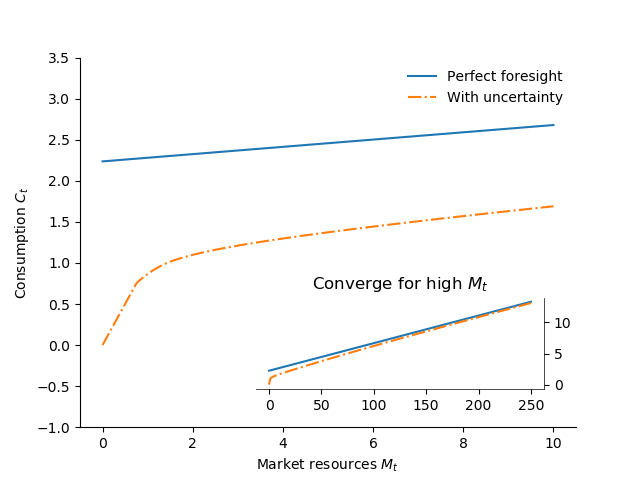
\includegraphics{./consumption_functions.png}
\caption{Consumption Functions\label{fig:consumption-functions}}
\end{figure}

\subsection{Macroeconomics: the Market
Class}\label{macroeconomics-the-market-class}

The modeling framework of \texttt{AgentType} is called ``microeconomic''
because it pertains only to the dynamic optimization problem of
individual agents, treating all inputs of the problem from their
environment as exogenously fixed. In what we label as ``macroeconomic''
models, some of the inputs for the microeconomic models are endogenously
determined by the collective states and choices of other agents in the
model. In a rational dynamic general equilibrium, there must be
consistency between agents' beliefs about these macroeconomic objects,
their individual behavior, and the realizations of the macroeconomic
objects that result from individual choices.

The Market class in \texttt{HARK.core} provides a framework for such
macroeconomic models, with a \texttt{solve} method that searches for a
rational dynamic general equilibrium. An instance of \texttt{Market}
includes a list of \texttt{AgentTypes} that compose the economy, a
method for transforming microeconomic outcomes (states, controls, and/or
shocks) into macroeconomic outcomes, and a method for interpreting a
history or sequence of macroeconomic outcomes into a new ``dynamic
rule'' for agents to believe. Agents treat the dynamic rule as an input
to their microeconomic problem, conditioning their optimal policy
functions on it. A dynamic general equilibrium is a fixed point dynamic
rule: when agents act optimally while believing the equilibrium rule,
their individual actions generate a macroeconomic history consistent
with the equilibrium rule.

\subsubsection{Down on the Farm}\label{down-on-the-farm}

The \texttt{Market} class uses a farming metaphor to conceptualize the
process for generating a history of macroeconomic outcomes in a model.
Suppose all \texttt{AgentTypes} in the economy believe in some dynamic
rule (i.e.~the rule is stored as attributes of each \texttt{AgentType},
which directly or indirectly enters their dynamic optimization problem),
and that they have each found the solution to their microeconomic model
using their \texttt{solve} method. Further, the macroeconomic and
microeconomic states have been reset to some initial orientation.

To generate a history of macroeconomic outcomes, the \texttt{Market}
repeatedly loops over the following steps a set number of times:

\begin{enumerate}
\def\labelenumi{\arabic{enumi}.}
\tightlist
\item
  \texttt{sow}: Distribute the macroeconomic state variables to all
  \texttt{AgentTypes} in the market.
\item
  \texttt{cultivate}: Each \texttt{AgentType} executes their
  \texttt{marketAction} method, likely corresponding to simulating one
  period of the microeconomic model.
\item
  \texttt{reap}: Microeconomic outcomes are gathered from each
  \texttt{AgentType} in the market.
\item
  \texttt{mill}: Data gathered by \texttt{reap} is processed into new
  macroeconomic states according to some ``aggregate market process''.
\item
  \texttt{store}: Relevant macroeconomic states are added to a running
  history of outcomes.
\end{enumerate}

This procedure is conducted by the \texttt{makeHistory} method of
\texttt{Market} as a subroutine of its \texttt{solve} method. After
making histories of the relevant macroeconomic variables, the market
then executes its \texttt{calcDynamics} function with the macroeconomic
history as inputs, generating a new dynamic rule to distribute to the
\texttt{AgentTypes} in the market. The process then begins again, with
the agents solving their updated microeconomic models given the new
dynamic rule; the \texttt{solve} loop continues until the ``distance''
between successive dynamic rules is sufficiently small.

\begin{comment}
\subsubsection{Sample Model: Fashion
Victim}\label{sample-model-fashion-victim}

We illustrate the \texttt{Market} class with a summary of an example from the full \href{https://github.com/econ-ark/HARK/blob/master/Documentation/HARKmanual.pdf}{HARK manual}. To illustrate the \texttt{Market} class consider a simple example in the emerging economic sub-field of aesthemetrics, the \texttt{FashionVictimModel}. This model is inspired by the paper \href{https://arxiv.org/abs/1410.8001v1}{``The hipster effect: When anticonformists all look the same'' by Jonathan Touboul}.\footnote{The \href{https://github.com/econ-ark/HARK/blob/master/Documentation/HARKmanual.pdf}{HARK manual} outlines the full problem and solution method in much more detail than the summary provided here. For a more traditional macroeconomic model, the \texttt{ConsAggShocksModel} module includes a consumption-saving model with both idiosyncratic and aggregate shocks, in which individual asset holdings are aggregated into total productive capital, endogenizing the interest and wage rate.}

Each period, fashion victims make a binary choice of style \(s\): to
dress as a jock (0) or punk (1). They receive utility directly from the
outfit they wear and as a function of the proportion of the population
who \emph{just wore} the same style; they also pay switching costs
(\(c_{pj}\),\(c_{jp}\)) if they change styles rather than keep the same
as the previous period.

The search for a dynamic general equilibrium is implemented in HARK's
\texttt{Market} class. The \texttt{marketAction} method of
\texttt{FashionVictimType} simulates one period of the microeconomic
model: each agent receives style preference shocks \(\eta_0\) and
\(\eta_1\), sees the current proportion of punks \(p_t\) (sown to them
as \texttt{pNow}), and chooses which style to wear.

When the \texttt{solve} method is run, the solver successively solves
each agent's microeconomic problem conditional on their beliefs about
the next periods, runs the \texttt{makeHistory} method to generate a
1000 period history of \(p_t\), and calculates a new punk belief rule
based on this history. This entire process is repeated until the solver
terminates when consecutive belief rules differ by less than 0.01 in any
dimension. \mbox{Figure \ref{fig:fraction-of-punks}} shows the fraction
of punks in the population over time after the model is
solved.\footnote{Smoothed with 25-period moving average.}

\begin{figure}
\centering
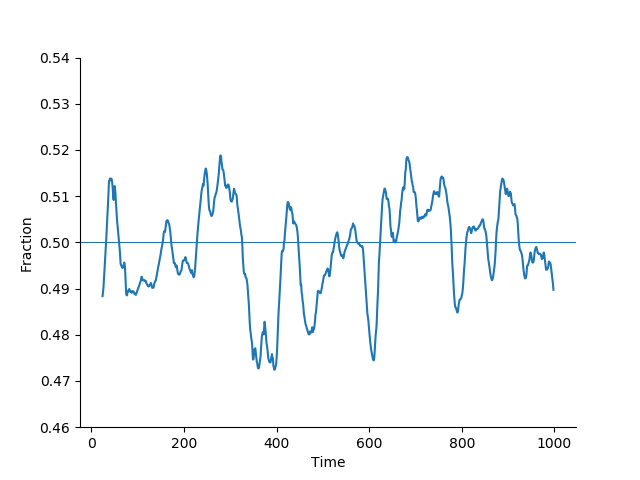
\includegraphics{./fraction_of_punks.png}
\caption{Fraction of Punks in Population over
Time\label{fig:fraction-of-punks}}
\end{figure}
\end{comment}

\begin{comment}
\section{\texorpdfstring{Tools from Software Development
\label{sec:tools-from-software-development}}{Tools from Software Development }}\label{tools-from-software-development}

One of the most striking practices to emerge from the history of
software development is the open open-source software moement: the
decentralized collaboration of many independent programmers on a single
project, often with little or no immediate monetary reward. Along with
fascinating theoretical questions about incentive structures, the
open-source movement has spurred the development of a wide array of
excellent utilities that make decentralized code development robust and
efficient. This section briefly overviews a number of tools from
traditional and open-source software development that enable
collabortion between researchers in many places.

\subsection{Documentation}\label{documentation}

Good documentation is the key to communication between two programmers,
whether between two distinct individuals or with oneself over time. In
Python, as in many scripting languages, strings written on the first
line after a function declaration are automatically employed as system
documentation. HARK currently uses a slight variation on the
\href{https://www.python.org/dev/peps/pep-0257/}{PEP 257} style guide.

In addition to traditional code documentation described above,
notebook-style interfaces similar to those in Mathematica and Maple
allow scientific programmers to directly communicate math ideas, and
code in a single place. The HARK project uses
\href{https://jupyter.org/}{Jupyter}, a language-agnostic, browser-based
notebook system spun off of the the IPython project.

\subsection{Unit Testing}\label{unit-testing}

Many programs are composed of a number of small functions that
accomplish specific tasks. Testing at the individual function level is
key to ensuring that the overall program executes correctly. This is all
the more important for scientific computing, where a mistake deep in the
code (eg. with a numerical approximation) may be extremely difficult to
track down. Unit testing is the formal practice whereby each individual
function is directly bundled with a set of tests. In scientific
programming, this can serve an additional purpose: peer review of code.
Uncovering bugs in code, even one's own code, can be notoriously
difficult. This is many times more true when one is examining the code
written by another.

Unit testing can ease the burden of scientific code review in at least
two ways. First, it can aid documentation in immediately outlining
simple examples of code execution. Second, it can outline the pitfalls
and testing procedures a reviewer may want to undertake to ensure that
the code is correct. Instead of starting with a ``blank page,'' a
reviewer can take the unit tests written by the original author, run
them, and then (assuming they all pass), examine the tests to see if any
particular cases appear to be excluded. If so, the reviewer can use the
unit tests as a template to quickly write another test case and run that
as well. This can greatly accelerate both the verification of work done,
as well as new testing of the code, all in a well-established and
minimally costly framework.

In Python there are two built-in ways to write tests for a function:
internally to the documentation, in a
``\href{https://docs.python.org/2/library/doctest.html}{doctest},'' and
externally in a more formal unit testing framework,
``\href{https://docs.python.org/2/library/unittest.html}{unittest}.''
HARK employs both where appropriate.

\subsection{Application Programming Interface
(API)}\label{application-programming-interface-api}

When contributing a module or a function to a larger code library, a
programmer needs to know how this function or module fits into the
overall framework of the codebase. Any large computational project with
multiple developers can benefit from an Application Programming
Interface (API). This is simply another form of language documentation,
but one that is aimed at programmers for extending or using a codebase.

The HARK project forms an API for the codebase organized around the
modules required to run a partial-equilibrium or general-equilibrium
estimation. Specifically, the simple API employed by the HARK defined by
the main functions and data structures employed in the Estimation
module, which is displayed and discussed in greater detail below. To
extend the HARK library the user must replace or otherwise replicate
these main functions in the Estimation module.\footnote{A further use of
  APIs is to define an interface between a programming language and a
  particular dataset. This second use of APIs is just as important as
  its usage in organizing code. Organizations such as the
  \href{http://openeconomics.net/}{Open Economics Working Group} may
  provide a unified approach for public economic datasets, but this is
  not part of HARK yet.}

\subsection{Version Control}\label{version-control}

An essential tool in distributed software development is a system that
can automatically archive versions of code, as well as allow the merging
of changes to a document by two different programmers. Such a system is
known as a version control system. The HARK project uses the Git version
control system, and uses the popular online repository service Github to
archive its codebase. Chacon and Straub
(\protect\hyperlink{ref-chacon2014pro}{2014}) is an excellent overview
of version control in general and Git and Github in particular. {]}

\subsection{Bringing It Together: Reproducible
Research}\label{bringing-it-together-reproducible-research}

Many of the tools above are used to create research that can be
immediately reproduced, even entirely in a web browser. This
\href{https://github.com/ipython/ipython/wiki/A-gallery-of-interesting-IPython-Notebooks}{gallery
of interesting IPython Notebooks} outlines a number of research projects
that combine code, discussion, data visualization, and descriptive
mathematics to make science as transparent and reproducible as possible.
For example Ram and Hadany
(\protect\hyperlink{ref-ram2015probability}{2015}) reproduce a section
of their work in an IPython notebook, which can be found
\href{http://nbviewer.ipython.org/url/www.sciencedirect.com/science/MiamiMultiMediaURL/1-s2.0-S0040580914000811/1-s2.0-S0040580914000811-mmc1.txt/272364/FULL/S0040580914000811/471cf02085a52c248dc76ae65ad4409d/mmc1.txt}{here}.

\end{comment}

\section{\texorpdfstring{Summary and Conclusion
\label{sec:summary-conclusion}}{Summary and Conclusion }}\label{summary-and-conclusion}

The HARK project is a modular code library for constructing
microeconomic and macroeconomic models with heterogeneous agents.
Portfolio choice under uncertainty is central to nearly all academic
models, including modern DSGE models (with and without financial
sectors), models of asset pricing (eg. CAPM and C-CAPM), models of
financial frictions (eg. Bernanke et al. 1999), and many more. Under
strict assumptions many of these models can be solved by aggregating
agent decision-making and employing the representative agent. However
when individual agents look very different from one another - for
example, different wealth levels, preferences, or exposures to different
types of shocks - assumptions required for aggregation can quickly fail
and a representative agent is no longer appropriate. Code to solve the
required heterogeneous-agent models tends to be bespoke and
idiosyncratic, often reinvented by different researchers working on
similar problems. This needless code duplication increases the chance
for errors and wastes valuable researcher time.

Researchers should spend their valuable time producing research, not reinventing wheels. The HARK toolkit already provides a useful set of industrial strength, reliable, reusable  wheels, constructed using a simple and easily extensible framework with clear documentation, testing, and estimation frameworks.  The longer-term goals of the Econ-ARK project are to create a collaborative codebase that can serve the entire discipline of economics, employing the best of modern software development tools to accelerate understanding and implementation of cutting edge research tools. The solution methods employed in HARK are not the only methods available, and those who have additional methodological suggestions are strongly encouraged to contribute! Increasing returns to production is one of the few ``non-dismal'' possibilities in economic thought -- we hope to capture this feature of code production in the HARK framework. Key next steps include finalizing the general-equilibrium HARK modules, identifying additional baseline models to replicate in HARK, and encouraging a new generation of students to learn from, use, and contribute to the collaborative construction of heterogeneous-agent models.

\section*{Bibliography}\label{bibliography}
\addcontentsline{toc}{section}{Bibliography}

\hypertarget{refs}{}
\hypertarget{ref-adjemian2011dynare}{}
Adjemian, Stéphane, Houtan Bastani, Michel Juillard, Ferhat Mihoubi,
George Perendia, Marco Ratto, and Sébastien Villemot. 2011. ``Dynare:
Reference Manual, Version 4.'' Dynare working papers 1, CEPREMAP.

\hypertarget{ref-aruoba2015comparison}{}
Aruoba, S Borağan, and Jesús Fernández-Villaverde. 2015. ``A Comparison
of Programming Languages in Macroeconomics.'' \emph{Journal of Economic
Dynamics and Control} 58. Elsevier: 265--73.

\hypertarget{ref-carroll2012implications}{}
Carroll, Christopher D. 2012. ``Implications of Wealth Heterogeneity for
Macroeconomics.'' \emph{Johns Hopkins University Department of Economics
Working Paper}, no. 597.

\hypertarget{ref-carroll2014representing}{}
---------. 2014a. ``Representing Consumption and Saving Without a
Representative Consumer.'' In \emph{Measuring Economic Sustainability
and Progress}, 115--34. University of Chicago Press.

\hypertarget{ref-kmvHANK}{}
---------. 2017. ``Monetary Policy According to HANK.'' In \emph{American Economic Review}, 697-743. 

\hypertarget{ref-carroll2014imfheterogeneousagentmacro}{}
---------. 2014b. ``Heterogeneous Agent Macroeconomics: An Example and
an Agenda.'' Washington, D.C.: Presentation at IMF Workshop on
Computational Macroeconomics.

\hypertarget{ref-carroll2017harkmanual}{}
Carroll, Christopher, Alexander Kaufman, David Low, Nathan Palmer, and
Matthew White. 2017. ``A User's Guide for Hark: Heterogeneous Agents
Resources and toolKit.''
\url{https://github.com/econ-ark/HARK/blob/master/Documentation/HARKmanual.pdf}:
Econ ARK.

\hypertarget{ref-carroll2017distribution}{}
Carroll, Christopher, Jiri Slacalek, Kiichi Tokuoka, and Matthew N
White. 2017. ``The Distribution of Wealth and the Marginal Propensity to
Consume.'' \emph{Quantitative Economics} 8 (3). Wiley Online Library:
977--1020.

\hypertarget{ref-chacon2014pro}{}
Chacon, Scott, and Ben Straub. 2014. \emph{Pro Git}. Apress.

\hypertarget{ref-geanakoplos2010leverage}{}
Geanakoplos, John. 2010. ``The Leverage Cycle.'' \emph{NBER
Macroeconomics Annual} 24 (1). The University of Chicago Press: 1--66.

\hypertarget{ref-geanakoplos2012getting}{}
Geanakoplos, John, Robert Axtell, J Doyne Farmer, Peter Howitt, Benjamin
Conlee, Jonathan Goldstein, Matthew Hendrey, Nathan M Palmer, and
Chun-Yi Yang. 2012. ``Getting at Systemic Risk via an Agent-Based Model
of the Housing Market.'' \emph{American Economic Review} 102 (3):
53--58.

\hypertarget{ref-ram2015probability}{}
Ram, Yoav, and Lilach Hadany. 2015. ``The Probability of Improvement in
Fisher's Geometric Model: A Probabilistic Approach.'' \emph{Theoretical
Population Biology} 99. Elsevier: 1--6.

\hypertarget{ref-sheppard2018introduction}{}
Sheppard, Kevin. 2018. ``Introduction to Python for Econometrics,
Statistics and Numerical Analysis.'' \emph{Lecture Notes, University of
Oxford}. \url{https://www.kevinsheppard.com/Python_for_Econometrics}.


\end{document}

\message{ !name(ccarroll_et_al_scipy_2018.tex) !offset(-789) }
